%!TEX root = ../../beamer.tex
\begin{frame}
\frametitle{stochasticity in gene expression}
\begin{center}
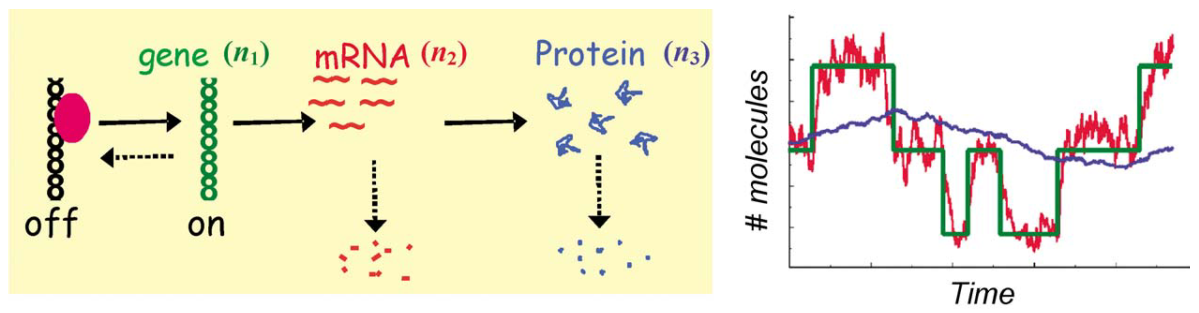
\includegraphics[width=0.9\textwidth]{fig/stochgeneexpdyn.png}\\
\end{center}
{\scriptsize
$n_1$ number of active genes, $n_2$ number of mRNAs, $n_3$ proteins per cell
\begin{align*}
\frac{P(n_1,n_2,n_3)}{dt} = &\lambda_1^+ (n_1^{max}-n-1 + 1)P(n_1 - 1,n_2,n_3) -\lambda_1^+ (n_1^{max}-n-1)P(n_1,n_2,n_3)\\
&+\lambda_1^- (n_1 + 1)P(n_1 + 1,n_2,n_3) -\lambda_1^- n_1 P(n_1,n_2,n_3)\\
&+\lambda_2 n_1P(n_1,n_2-1,n_3) - \lambda_2 n_1 P(n_1,n_2,n_3)\\
&+(n_2+1)/\tau_2 P(n_1,n_2+1,n_3) - n_2/\tau_2P(n_1,n_2,n_3)\\
&+\lambda_3 n_2 P(n_1,n_2,n_3 - 1) - \lambda_3 n_2 P(n_1,n_2,n_3)\\
&+(n_3 + 1)/\tau_3 P(n_1,n_2,n_3+1) - n_3/\tau_3 P(n_1,n_2,n_3)
\end{align*}}
\end{frame}
